%!TEX root = ../../../../report.tex
\subsection{Limb profile} % (fold)
\label{sub:limb_profile}
Based on the requirements of weight and its distribution defined in the analysis of the joints \ref{sec:joints}, the links have been decided to have in the upper extreme the actuators. 
This leads to use a transmission system, such as belt and pulleys, which leaves for the rest of link a structural function that can also adopt the task of wiring placement.
Thus, a light weight section that satisfy the conditions of deformation and stress maximum will be chosen.
Carbon fiber is an ideal material to achieve these conditions of weight and stress so an quantitative analysis has been made calculating the optimal solution and then rounding it for all the possible profiles offered by the given provider.
The provider was chosen due to previous experiences that the Mærsk Mc-Kinney Møller Institute had with carbon fiber orders.

The section profile offered\footnote{http://www.easycomposites.co.uk/\#!/cured-carbon-fibre-products/} are: \textit{Rod}, \textit{Tube}, \textit{Box}. The \textit{Stripe} and the \textit{Angle} are discarded due to its asymmetrical geometry that will will lead to less predictable scenarios.
The study case is show in the figure \ref{fig:impact_decomposition}, where the impact force can be decomposed in a pure bending effort and a pure compression.
Due to the resistance of the carbon fiber in pure compression is bigger than in bending, only this last case has been studied.
This studies should not completly follow the behaviour in real life due to the carbon fiber is not an isomorphic material.
However, the high security factor taken into account is expected to overcome this assumption.

\begin{figure}[ht!]
  \centering
  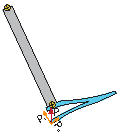
\includegraphics[width=.3\textwidth]{figures/impact_decomposition.pdf}
  \caption{Impact force decomposed}
  \label{fig:impact_decomposition}
\end{figure}

\subsubsection{Profile study} % (fold)
\label{ssub:profile_study}
  The bending effort causes two sort of problems: (1) the possible break in the supporting point and (2) the deformation suffered by the beam.
  The break will occur when the tensions created will be over the ultimate tension in compression or tension of the selected material.
  This comes defined in the equation \ref{eq:tension} for symmetric sections and when an only torque is being applied.
  \begin{equation}
  \label{eq:tension}
    \sigma _{compression} = \sigma _{tension} = \frac{M h_{CG}}{I_x}
  \end{equation}

  Meanwhile the deformation in the extreme can be calculated with the equation \ref{eq:deformation} if the case is simplified to the occurred in the figure \ref{fig:bending_case}.
  This is, when the leg is completely stretched, what will cause the biggest stresses.

  \begin{figure}[ht!]
    \centering
    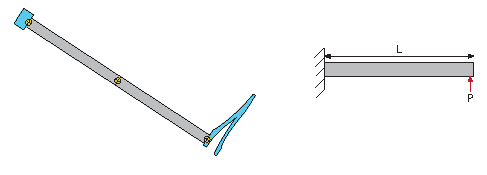
\includegraphics[width=\textwidth]{figures/bending_case.pdf}
    \caption{Simplified representation of the bending case}
    \label{fig:bending_case}
  \end{figure}

  \begin{equation}
  \label{eq:deformation}
    y_L = \frac{P z^2}{6EI}(3L-z) = \frac{P L^2}{6EI}(2L) = \frac{P L^2}{3EI}
  \end{equation}


  For the selected profiles the equations that define the compression ($\sigma _{compression}$) and tension efforts ($\sigma _{tension}$), along with the deformation in the direcction of the applied force ($y_L$) are shown, being:

  \begin{enumerate}
    \item $h_{CG}$: height of the center of gravity of the semi-half section from the geometrical center of the section.

    \item $E$: Elastic module.
  \end{enumerate}


  \noindent\begin{minipage}{0.2\textwidth}% adapt widths of minipages to your needs
      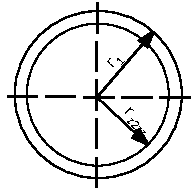
\includegraphics[width=\linewidth]{figures/profile_cylinder.pdf}
  \end{minipage}%
  \hfill%
  \begin{minipage}{0.8\textwidth}
    \begin{equation}
      \begin{aligned}
      \sigma _{compression} = \sigma _{tension} &= \frac{M h_{CG}}{I_x} = \frac{4 r_2}{\pi(r_2 ^4 - r_1 ^4)} M \\
      y_L &= \frac{P L^2}{3EI} = \frac{4 P L^2}{3 E \pi(r_2 ^4 - r_1 ^4)}\\
      h_{CG} &= r_2 \\
      I_x = I_y &= \frac{\pi}{4} (r_2 ^4 - r_1 ^4)
      \end{aligned}
    \end{equation}
  \end{minipage}

  \noindent\begin{minipage}{0.2\textwidth}% adapt widths of minipages to your needs
      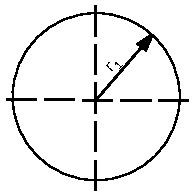
\includegraphics[width=\linewidth]{figures/profile_tube.pdf}
  \end{minipage}%
  \hfill%
  \begin{minipage}{0.8\textwidth}
    \begin{equation}
    \begin{aligned}
      \sigma _{compression} = \sigma _{tension} &= \frac{M h_{CG}}{I_x} = \frac{4}{\pi r_1 ^3} M\\
      y_L &= \frac{P L^2}{3EI} = \frac{4 P L^2}{3 E \pi r_1 ^4}\\
      h_{CG} &= r_1 \\
      I_x = I_y &= \frac{\pi r_1 ^4}{4}
      \end{aligned}
    \end{equation}
  \end{minipage}

  \noindent\begin{minipage}{0.2\textwidth}% adapt widths of minipages to your needs
      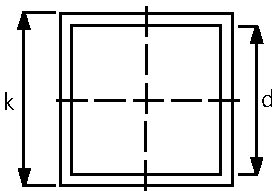
\includegraphics[width=\linewidth]{figures/profile_squared.pdf}
  \end{minipage}%
  \hfill%
  \begin{minipage}{0.8\textwidth}
    \begin{equation}
    \begin{aligned}
      \sigma _{compression} = \sigma _{tension} &= \frac{M h_{CG}}{I_x} = \frac{6 d}{(d^4 - k^4)}\\
      h_{CG} &= \frac{d}{2} \\
      y_L &= \frac{P L^2}{3EI} = \frac{4 P L^2}{E (d^4 - k^4)}\\
      I_x = I_y &= \frac{1}{12} (d^4 - k^4)
      \end{aligned}
    \end{equation}
  \end{minipage}
% subsubsection profile_study (end)

\subsubsection{Torque calculation} % (fold)
\label{ssub:torque_calculation}
  For both cases, the profile of the lower limb and the upper, the torque generated by the impact force determined in the section \ref{sub:impact_force}, is calculated.
  This torque is different in the lower and the upper limb due to the upper limb takes the distance from the foot to the hip while the other one is only from the foot to the knee:
  \begin{equation}
  \begin{aligned}
     M_{lower\ limb} = F \cdot d = 294.4 \cdot 0.2126 = 62.57 Nm\\
     M_{upper\ limb} = F \cdot d = 294.4 \cdot (0.2126 + 0.2622) = 139.73 Nm
  \end{aligned}
  \end{equation}
% subsubsection torque_calculation (end)

\subsubsection{Final limb parameters} % (fold)
\label{ssub:final_limb_parameters}
Following the criteria from the sections \ref{sec:dimensions} and \ref{sec:physical_properties} of size and materials, the presented formulas and the have been applied to all the profiles of the provider.
An iterative process based on the outputs of the mathematical model \ref{cha:mathematical_model} has given as a result the limb lengths shown in the table \ref{tab:limb_lengths}.

\begin{table}[ht!]
\centering
\caption{Final limb lengths}
\label{tab:limb_lengths}
\begin{tabular}{r|l}
  \textbf{Limb} & \textbf{Length [m]} \\ \hline
  Foot length & 0.095 \\ \hline
  Foot width & 0.030 \\ \hline
  Lower limb & 0.212 \\ \hline
  Upper limb & 0.262 \\ \hline
  Hip width & 0.150     
\end{tabular}
\end{table}

Then, the profiles have been analyzed calculating the torque from \ref{ssub:torque_calculation} and then applying the section \ref{ssub:profile_study} for each iteration.
The calculations of the last iteration are shown in the appendix \ref{app:profile_selection}.
These results have been then approved or discarded based on a \textit{maximum deformation} and \textit{ultimate tension} requirements, and are shown in the table \ref{tab:profile_selection}

\begin{table}[ht!]
\centering
\caption{Profile selection for each limb}
\label{tab:profile_selection}
\begin{tabular}{c|c|c}
  \textbf{Limb} & \textbf{Section} & \textbf{Dimensions} \\ \hline
  Lower limb & Tube & 20 mm and 1 mm thickness \\ \hline
  Upper limb & Tube & 20 mm and 1 mm thickness 
\end{tabular}
\end{table}

% subsubsection profile_selection (end)



% subsection limb_profile (end) 